\documentclass[]{politex-xico}



% ========== Packages ==========
\usepackage[utf8]{inputenc}
\usepackage{amsmath,amsthm,amsfonts,amssymb}
\usepackage{graphicx,cite,enumerate}
\usepackage{multirow}
\usepackage[ruled,vlined]{algorithm2e}
\usepackage{pdfpages}
%\usepackage{natbib}
\usepackage{amsmath,amssymb,mathtools}
\DeclareMathOperator*{\argmax}{arg,max}
\usepackage{todonotes}
\usepackage{booktabs,tabularx}
\usepackage[normalem]{ulem}
\usepackage[alf,abnt-etal-list=0]{abntex2cite-xico}
% ========== Language options ==========
%\usepackage[brazil]{babel}
\usepackage[english]{babel}
\usepackage[table,xcdraw]{xcolor}

% ========== ABNT (requer ABNTeX 2) ==========
%	http://www.ctan.org/tex-archive/macros/latex/contrib/abntex2
%\usepackage[num]{abntex2cite}

% Forçar o abntex2 a usar [ ] nas referências ao invés de ( )
%\citebrackets{[}{]}


% ========== Lorem ipsum ==========
\usepackage{blindtext}



% ========== Opções do documento ==========
% Título
\titulo{Noise-Gated Retrieval: Embedding-Based
Context Compression for Cost-Aware RAG}

% Autor
\autor{ARNOLD ALVARO MOYA LAVADO}

% Orientador / Coorientador
\orientador{Prof. Dr. Anna Helena Reali Costa}
%\coorientador{Nome do coorientador (opcional)}

% Tipo de documento
%\tcc{Eletricista com ênfase em Sistemas Eletrônicos}
%\dissertacao{Electrical Engineering}
\teseDOC{Electrical Engineering}
%\teseLD
%\memorialLD

% Departamento e área de concentração
\departamento{Computação e Sistemas Digitais - PCS}
\areaConcentracao{Computer Engineering}

% Local
\local{São Paulo}

% Ano
\data{2025}




\begin{document}
% ========== Capa e folhas de rosto ==========
\capa
\falsafolhaderosto
\folhaderosto


% ========== Folha de assinaturas (opcional) ==========
%\begin{folhadeaprovacao}
%	\assinatura{Prof.\ X}
%	\assinatura{Prof.\ Y}
%	\assinatura{Prof.\ Z}
%\end{folhadeaprovacao}


% ========== Ficha catalográfica ==========
%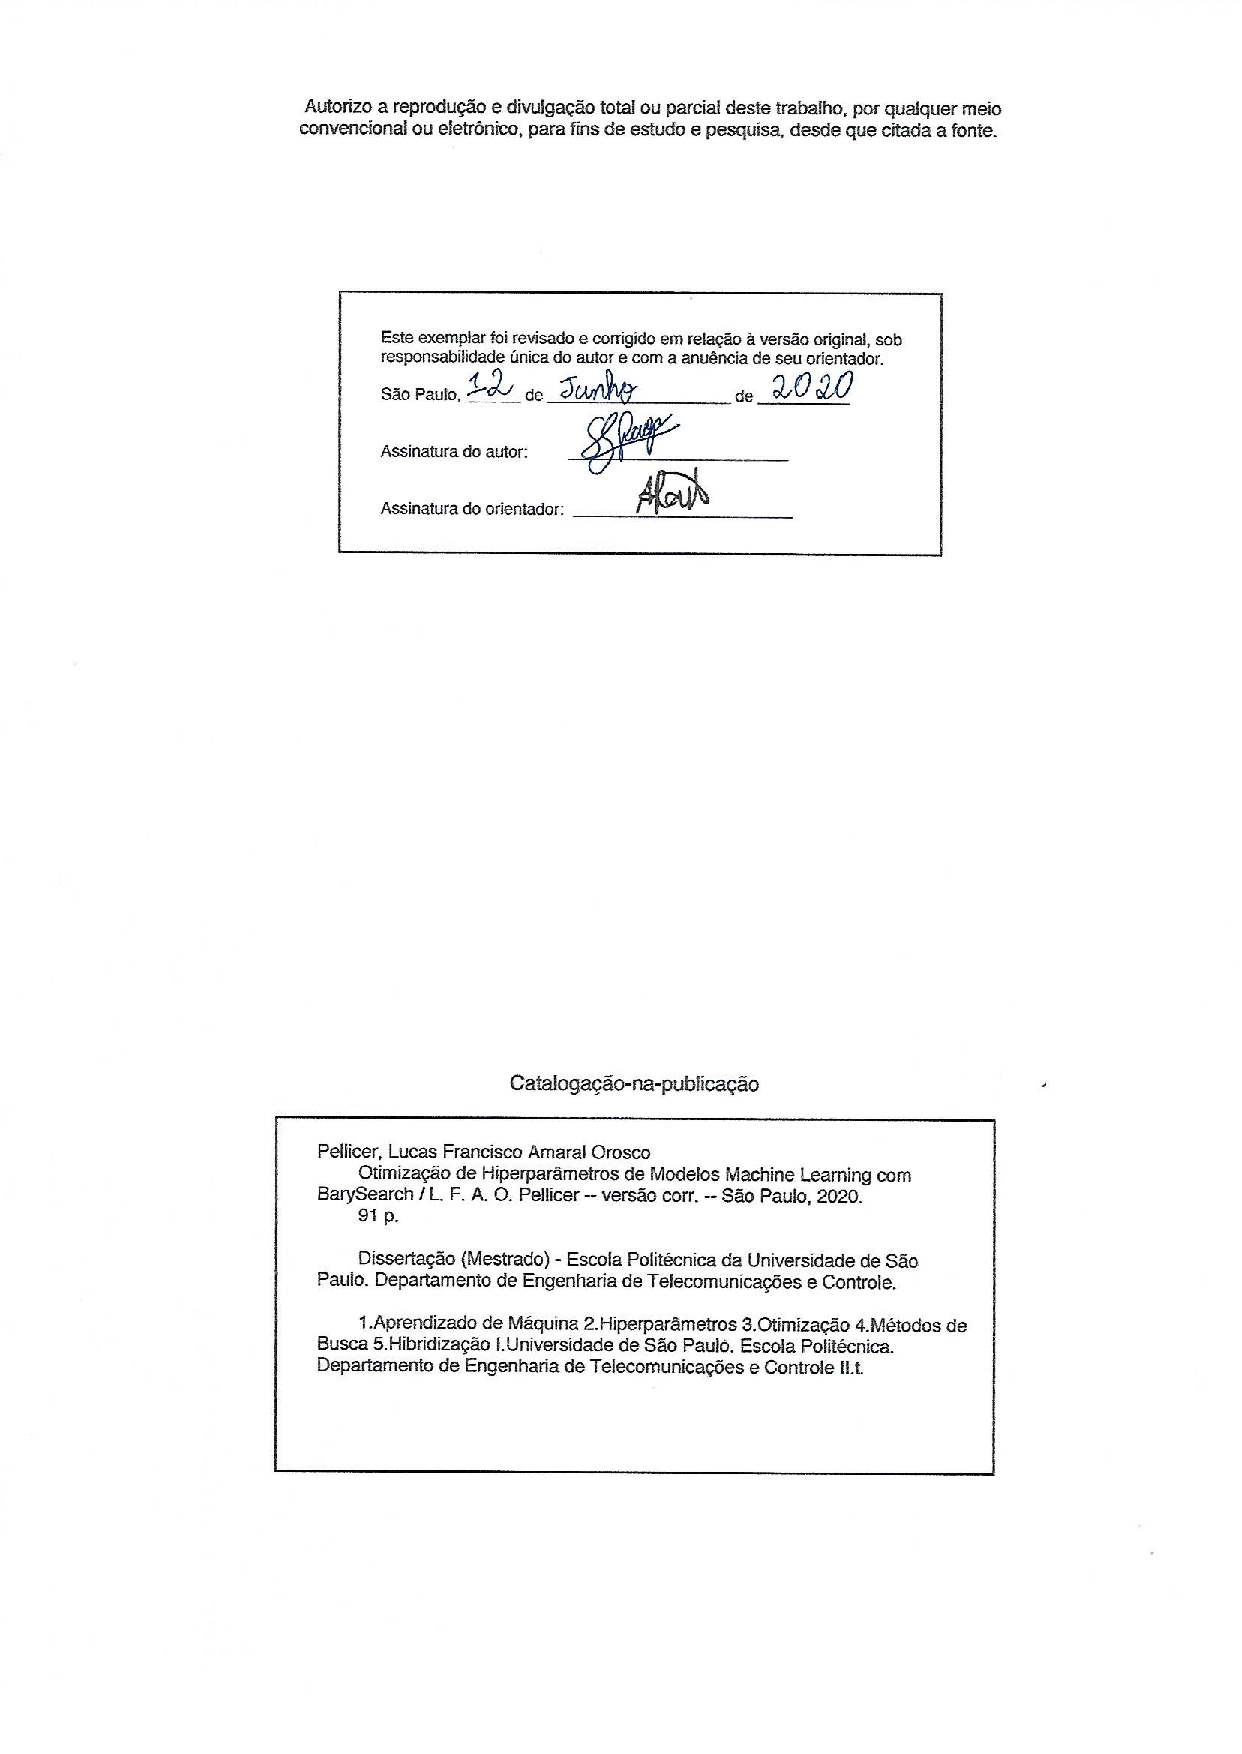
\includepdf[pages=-]{catalagacao-epusp-final}
% Fazer solicitação no site:
%	http://www.poli.usp.br/en/bibliotecas/servicos/catalogacao-na-publicacao.html


% ========== Dedicatória (opcional) ==========
%\dedicatoria{Dedico esse trabalho à minha mãe, Rosanna e ao meu pai, Francisco, por todo ensinamento, inspiração, auxílio, carinho e orientação. Também para minhas avós (Irene e Ignês) e avôs (Antônio e Walter), além de tias e tios e aos meus amigos Mike e Jimmy que sempre deram alegria.}


% ========== Agradecimentos ==========
\begin{agradecimentos}
I want to thank the Universidade de São Paulo (USP), the graduate program in Electrical Engineering at the Escola Politécnica (PPGEE), and the Coordination for the Improvement of Higher Education Personnel (CAPES, Finance Code 001) for supporting this work. I also thank the supervisor Prof. Anna Helena Reali Costa, once again, for her patience, guidance, and willingness to teach. Finally, thanks also to my colleagues for their support in so many discussions and a few papers during the development of the work.

\end{agradecimentos}


% ========== Epígrafe (opcional) ==========
%\epigrafe{%
%	\emph{``Epígrafe''}
%	\begin{flushright}
%		E, se bem que seja obscuro\\
%Tudo pela estrada fora,\\
%E falso, ele vem seguro,\\
%E, vencendo estrada e muro,\\
%Chega onde em sono ela mora.\\
%E, inda tonto do que houvera,\\
%A cabeça, em maresia,\\
%Ergue a mão, e encontra hera,\\
%E vê que ele mesmo era A Princesa que dormia.\\
%\textit{Fernando Pessoa}
%	\end{flushright}
%}


% ========== Resumo ==========
\begin{resumo}
A classificação de textos em regime \textit{zero-shot} frequentemente troca usabilidade por acurácia: os melhores resultados dependem de modelos muito grandes e hardware custoso, enquanto métodos eficientes com modelos pequenos tipicamente requerem dados rotulados. Apresentamos o ZeroBERTo 2.0, um pipeline concebido para baixo recurso que aprende exclusivamente a partir de dados não rotulados e executa em hardware de consumo. A abordagem baseia-se em Sentence Transformers compactos, como o SetFit, e adapta o ajuste fino contrastivo do SetFit ao regime \textit{zero-shot} via auto-treinamento: o modelo gera pseudo-rótulos, filtra-os com um sinal explícito de qualidade e seleciona um subconjunto balanceado e diverso para refinar-se iterativamente — sem anotação humana. Em múltiplos conjuntos de dados públicos que abrangem sentimentos, tópicos e intenção, o ZeroBERTo 2.0 frequentemente iguala ou supera sistemas \textit{zero-shot} maiores baseados em implicação textual (\textit{entailment}) e recuperação, e se aproxima de métodos \textit{few-shot} fortes quando avaliado em seu melhor estágio de treinamento.
Entretanto, na ausência de dados de validação rotulados, a parada antecipada confiável é desafiadora: à medida que o auto-treinamento avança, o desempenho pode divergir e degradar, e observamos alta sensibilidade às escolhas de hiperparâmetros, que são dependentes do conjunto de dados. Consequentemente, uma implantação prática com desempenho consistente atualmente requer a seleção manual de hiperparâmetros por conjunto de dados para evitar colapso em iterações tardias. Documentamos esse fenômeno e enquadramos a seleção de modelos sem rótulos como um problema central em aberto para auto-treinamento \textit{zero-shot}. Apresentamos sinais iniciais, totalmente não supervisionados, para parada (por exemplo, calibração de confiança, tendências de entropia e concordância entre iterações) e estudamos a possibilidade de desenvolver critérios sólidos e bem fundamentados que determinem quando interromper o treinamento sem rótulos. Nossos resultados iniciais indicam que a curadoria cuidadosa de pseudo-rótulos — priorizando tanto a confiança quanto a diversidade — permite que modelos pequenos sejam competitivos em cenários \textit{zero-shot}, e que avançar em técnicas de parada antecipada sem rótulos é chave para tornar tais sistemas confiavelmente utilizáveis na prática.
%\\[3\baselineskip]

%
\textbf{Palavras-Chave} -- classificação de texto sem amostras, auto-treinamento, pseudo-rotulagem, seleção à base de diversidade.
\end{resumo}


% ========== Abstract ==========
\begin{abstract}
Zero-shot text classification often trades usability for accuracy: the strongest results rely on very large models and costly hardware, while efficient small-model methods typically require labeled data. We introduce ZeroBERTo 2.0, a low-resource-by-design pipeline that learns exclusively from unlabeled data and runs on consumer hardware. The approach builds on compact Sentence Transformers such as SetFit, and adapts SetFit’s contrastive fine-tuning to the zero-shot regime via self-training: the model generates pseudo-labels, filters them with an explicit quality signal, and selects a balanced, diverse subset to iteratively refine itself—without human annotation. Across multiple public datasets spanning sentiment, topic, and intent classification, ZeroBERTo 2.0 often matches or surpasses larger entailment and retrieval-style zero-shot systems and approaches strong few-shot methods when measured at its best training stage.
However, in the absence of labeled validation data, reliable early stopping is challenging: as self-training proceeds, performance can diverge and degrade, and we observe high sensitivity to hyperparameter choices that are dataset-dependent. Consequently, practical deployment with consistent performance currently requires cherry-picking hyperparameters per dataset to avoid late-iteration collapse. We document this phenomenon and frame label-free model selection as a central open problem for zero-shot self-training. We outline initial, fully unsupervised stopping signals (e.g., confidence calibration, entropy trends and cross-iteration agreement) and study the possibility of developing principled, robust criteria that determine when to stop training without labels. Our early results indicate that careful pseudo-label curation—prioritizing both confidence and diversity—enables small models to compete in zero-shot settings, and that advancing label-free early stopping is key to making such systems reliably usable in practice.

\textbf{Keywords:} zero-shot text classification, self-training, pseudo-labeling, diversity-aware selection, early stopping

\end{abstract}


% ========== Listas (opcional) ==========
\listadefiguras
\listadetabelas


\chapter*{{List of Acronyms}}
%\addcontentsline{toc}{chapter}{Lista de Símbolos}


% Preencha abaixo. É uma simples tabela.
\begin{table*}[h]
\begin{tabular}{  l  l } 
BERT  &  \textbf{B}idirectional \textbf{E}ncoder \textbf{R}epresentations from \textbf{T}ransformers\\
BERTimbau & Pretrained BERT models for Brazilian Portuguese\\
c-TF-IDF & class-based Term Frequency–Inverse Document Frequency\\
DA & Data Augmentation\\
FSL & Few-Shot Learning\\
GLUE & General Language Understanding Evaluation\\
GPU & Graphics Processing Unit\\
HDBSCAN & Hierarchical Density-Based Spatial Clustering of Applications with Noise\\
LDA & Latent Dirichlet Allocation\\
LLM & Large Language Model\\
LSTM & Long Short-Term Memory\\
MNLI & Multi-Genre Natural Language Inference\\
mBERT & Multilingual BERT\\
MIPS & Maximum Inner Product Search\\
MLM & Masked Language Modeling\\
MTEB & Massive Text Embedding Benchmark\\
NLI   & Natural Language Inference\\
NLP   & Natural Language Processing\\
Open-QA   & Open-Domain Question Answering\\
PEFT & Parameter-Efficient Fine-Tuning\\
PET & Pattern-Exploiting Training\\
PLM & Pretrained Language Model\\
RoBERTa   & Robustly Optimized BERT Approach\\
RC & Reading Comprehension\\
RALM & Retrieval Augmented Language Models\\
RLVR & Reinforced Learning with verificable rewards\\
SetFit & Sentence Transformer Fine-Tuning\\
SFT & Supervised Fine-Tuning\\
ST & Sentence Transformer\\
XLNet   & Generalized Autoregressive Pretraining for Language Understanding\\
XLM-R & Cross-lingual Language Model – RoBERTa\\
XNLI & Cross-lingual Natural Language Inference\\
ZSC & Zero-Shot (Text) Classification\\
ZSL & Zero-Shot Learning\\
ZeroBERTo & \textbf{Zero}-shot \textbf{BERT} based on \textbf{To}pic Modeling\\
\end{tabular}
\end{table*}


\chapter*{{List of Symbols}}
%\addcontentsline{toc}{chapter}{Lista de Símbolos}


% Preencha abaixo. É uma simples tabela.
\begin{table*}[h]
\begin{tabular}{  l  l } 
$\phi$   & Encoding of the Embedding Model\\
$C$  &  Set of all possible labels\\
$d$ & Dimensionality of the vector space\\
$D$ & Dataset\\
$key$   &  Keyword\\
$m$  &  Number of total labels\\
$n$  &  Number of samples per class for Few-Shot Learning \\
$N$ & Number of documents in Original Dataset\\
$R$  &  Number of triplets\\
$st$ & Sentence Transformer\\
$st_0$  &  Pretrained Sentence Transformer\\
$st'$  &  Trained Sentence Transformer\\
$U$ & Unlabeled documents (Dataset)\\
$T_{-}$  &  Triplets negative (documents of different labels)\\
$T_{+}$  &  Triplets positive (documents of the same label)\\
\end{tabular}
\end{table*}

% ========== Sumário ==========
\sumario


\chapter{Introduction}
\label{chapter:Introduction}

This work addresses low-resource zero-shot text classification: building usable classifiers without task-specific labels and under tight computational budgets. We focus on practical, small-model solutions that run on consumer hardware while remaining competitive with larger, entailment-based \cite{pamies2023weakly} or LLM-style zero-shot methods \cite{kojima2022large}. The outcome is \texttt{ZeroBERTo-2}, a lightweight pipeline that learns exclusively from unlabeled data via self-training with compact Sentence Transformers \cite{reimers2019sentence} and diversity-aware pseudo-label selection.

Large pretrained language models have made zero-shot classification increasingly effective, often by recasting classification as textual entailment or by prompting with label verbalizations. However, the strongest zero-shot results typically depend on models that are expensive to run and tune, and that assume prompt engineering or template design. In contrast, small Sentence Transformers paired with contrastive learning (e.g., SetFit \cite{setfit}) show strong efficiency and robustness, but traditionally require at least a handful of labeled examples per class. \texttt{ZeroBERTo-2} closes this gap by enabling small-model zero-shot learning: it starts from label names (or descriptions) as anchors, produces initial compatibility scores in an embedding space, mines high-quality and diverse pseudo-labels, and iteratively refines a compact encoder–classifier stack without any human annotation.


This chapter is organized as follows. Section \ref{sec:text_classification_problem} introduces the text classification problem under low-resource and zero-shot constraints and outlines limitations of current solutions. Section \ref{sec:motivation_goals} presents the motivation and states the main goals and contributions of this work. Section \ref{sec:text_organization} summarizes the remainder of the document.

\section{Text Classification Problem}
\label{sec:text_classification_problem}

Text classification maps an input document to one or more labels from a predefined set. Formally, given a collection of unlabeled texts $U=\{x_1,\dots,x_N\}$ and a label set $\mathcal{C}=\{c_1,\dots,c_m\}$, the task is to learn a function that scores or predicts the plausibility that $x_i$ belongs to $c_j$. Applications span sentiment and emotion analysis, topic categorization, intent detection, customer-support routing and many others.



Zero-shot classification assumes no labeled examples of the target classes \cite{yin2019benchmarking}. In NLP, a dominant approach reformulates classification as textual entailment, scoring whether a document entails a label-specific hypothesis \cite{obamuyide2018zero} Another family embeds documents and label names or descriptions in a shared vector space and classifies by similarity \cite{cho2024zero}. While effective, the former generally relies on large models with high memory and compute requirements and sensitivity to prompt or template choices; the latter can be efficient but often trails large-model performance unless supported by additional learning.


Our prior work explored two complementary directions. First \cite{alcoforado2022zeroberto}, we showed that small models benefit from structural preprocessing and representation learning, improving efficiency without relying on long-context architectures.  Second, \cite{alcoforado2024random,alcoforado2025estrategias}, we demonstrated that diversity-aware selection yields stronger few-shot sets than random sampling, especially under class imbalance. Building on these insights, \texttt{ZeroBERTo-2} targets true zero-shot learning with small models by combining label-name anchoring, pseudo-label self-training, and explicit diversity control—without human labels, prompts, or large GPUs.

\section{Motivation and Main Goals}
\label{sec:motivation_goals}

Collecting labeled data is expensive and slow, and crowdsourcing often introduces noise, bias, and class imbalance. Meanwhile, entailment-based and LLM-based zero-shot methods deliver strong accuracy but impose significant computational and operational costs, limiting deployment on consumer hardware. Efficient few-shot methods with Sentence Transformers bridge usability and performance but still require labeled seeds.

We pursue a practical path to zero-shot learning with small models:
\textbf{First}, leverage unlabeled corpora to bootstrap training from label names or descriptions;
\textbf{then}, generate pseudo-labels and select them to maximize both quality and diversity;
\textbf{after that}, refine compact encoders with contrastive objectives and train a lightweight classification head;
\textbf{finally}, investigate label-free signals for early stopping and model selection, improving stability without any validation labels.

The main contributions of this work are:

\begin{itemize}
    \item \texttt{ZeroBERTo-2}, a three-stage zero-shot pipeline: First-Shot scoring from label names, diversity-aware pseudo-label selection, and contrastive refinement, that adapts SetFit-style efficiency to the zero-label regime.
    \item A comprehensive evaluation showing that \texttt{ZeroBERTo-2} is competitive both against few-shot models and against larger zero-shot models while remaining deployable on consumer hardware and executable with one line of code.
    \item An investigation of unsupervised stopping criteria for label-free self-training, documenting common failure modes and proposing practical signals for stability.
\end{itemize}



\section{Text Organization}
\label{sec:text_organization}

The remainder of this document is organized as follows: Chapter 2 reviews related work on zero-shot text classification (entailment-based and embedding-based methods), self-training and pseudo-labeling, efficient few-shot learning with Sentence Transformers, and diversity-aware data selection.
Chapter 3 presents \texttt{ZeroBERTo-2}: problem setup, the end-to-end pipeline, First-Shot scoring, pseudo-label selection, contrastive refinement, inference, and label-free early stopping.
Chapter 4 details experimental design: datasets, baselines, metrics, ablations, and evaluation protocols for low-resource and zero-shot scenarios.
Chapter 5 reports results already achieved, analyzing performance, efficiency, robustness, and the behavior of the proposed stopping signals.
Chapter 6 discusses limitations, future work, and the schedule for the remaining stages of the research.


\chapter{Fundamentals and Overview of the Area}
\label{chapter:review}

This chapter reviews the literature relevant to low-resource and zero-shot text classification. We begin with general definitions of zero-shot and low-resource learning across domains and recall core notions about vector spaces and embeddings. We then cover modern zero-shot strategies for text (entailment-based and beyond), self-training with unlabeled data, topic modeling and clustering for compression of long inputs, efficient few-shot learning with Sentence Transformers, informed data selection for annotation, and considerations about multilinguality and long documents that motivate our design choices in \texttt{ZeroBERTo-2}.
%%%

\section{Foundations: Zero-Shot, Low-Resource, and Embedding Spaces}
\label{sec:foundations}

\subsection{Retrieval-Augmented Language: General Definitions}

Zero-shot learning refers to building a classifier for target classes without any task-specific labeled examples. Historically, zero-shot emerged in computer vision by leveraging attribute vectors or cross-modal label embeddings to recognize unseen categories \cite{socher2013zero,romera2015embarrassingly}. The key idea is to map both inputs and labels (or label descriptions) into a common semantic space and perform classification by compatibility (e.g., similarity) in that space. Few-shot learning, in turn, assumes a very small number of labeled instances per class. Low-resource NLP broadly covers scenarios with limited supervision due to rare domains or languages \cite{hedderich2020survey}.

In NLP, zero-shot classification rose to prominence with Pretrained Language Models (PLMs). One popular strategy recasts classification as textual entailment (also known as Natural Language Inference or NLI), in which the text is understood as two separate parts: a "premise" and a "hypothesis". The classification is carried out by choosing a hypothesis that makes sense given a premise, and this is usually done by prompting a NLI head with label verbalizations \cite{yin2019benchmarking,williams2018broad,BERT,liu2019roberta,conneau2018xnli}. For instance, "The new Pope was chosen yesterday." is a premise that entails the hypothesis "This text is about religion.", but does not entail "This text is about sports."  Alternatively, non-parametric and retrieval-based methods compare inputs against label names, descriptions, or prototypes without supervised finetuning. Large Language Models (LLMs) further enable in-context learning, often showing strong zero- or few-shot behavior out of the box \cite{brown2020language,chan2022data,liu2023summary}.

\subsection{Vector Spaces and Embeddings}
Let $\phi: \mathcal{X} \to \mathbb{R}^d$ be an encoder mapping texts to $d$-dimensional vectors. Similarity between vectors $x$ and $y$ in the embedding space (e.g., cosine) serves as a proxy for semantic relatedness:

\begin{equation}
    sim(x,y) \coloneqq
    \frac{\phi(x) \cdot \phi(y)}{\lVert \phi(x) \rVert  \lVert \phi(y) \rVert}.
\end{equation}
 

In zero-shot classification, we can define label embeddings from label names or their natural-language descriptions and classify a document $d$ via

\begin{equation}
    \hat{c}(d) \coloneqq
argmax_{c \in \mathcal{C}}
\bigl(\phi(d), \phi(\text{name}(c))\bigr),
\end{equation}
with $c$ 
or by using an entailment head that scores hypothesis templates for each label \cite{yin2019benchmarking}.

Modern contextual encoders (Transformers) produce token-level representations aggregated into document embeddings. Pretraining objectives (masked language modeling, next-sentence prediction, etc.) imbue these vectors with structure that correlates with semantics \cite{BERT,liu2019roberta,attentionallyouneed}. Sentence-level encoders evaluated on benchmarks such as MTEB \cite{muennighoff2023mteb} show that small, specialized models can provide robust embedding spaces for retrieval, clustering, and classification \cite{lee2024nvembed,duquenne2023sonar}. Contrastive finetuning (e.g., SetFit) further improves class separability by pulling same-class examples together and pushing different-class examples apart, even with very few labels \cite{setfit}.

Generally, we can trust Transformer-based embeddings to achieve some degree of semantic alignment: in these models, cosine similarity of sentence embeddings tends to correlate with semantic similarity tasks, while contrastive finetuning strengthens this alignment \cite{setfit,muennighoff2023mteb}. Also, label names or descriptions embedded in the same space often suffice to define class prototypes for zero-shot decisions \cite{yin2019benchmarking}.
Finally, we can also trust multilingual capabilities in most PLMs, as they align cross-lingual semantics, enabling transfer across languages with a single encoder \cite{multilingualbert,DBLP:journals/corr/abs-1911-02116,conneau2020unsupervised}.
These models, however, pose some limitations. For instance, long inputs stress fixed context windows \cite{beltagy2020longformer,Zaheer2020BigBT} and domain shift can degrade embedding reliability. But careful pooling and compression (e.g., topic modeling) can mitigate these issues.

\section{Zero-Shot Text Classification in NLP}
\label{sec:zs_tc}

Entailment-based zero-shot classification repurposes NLI heads to score whether a document entails each label hypothesis \cite{yin2019benchmarking,williams2018broad,conneau2018xnli}. While effective, these approaches face three practical hurdles: (i) computational and memory cost of large PLMs; (ii) handling of long documents and (iii) the need for manually crafting the "hypothesis template" for most pipelines. Long-context architectures alleviate truncation but remain relatively expensive \cite{beltagy2020longformer,Zaheer2020BigBT}. LLMs deliver strong zero- or few-shot performance via in-context learning \cite{brown2020language,chan2022data}, yet are often too large for consumer hardware.

Efficiency-oriented work explores non-parametric and data-efficient strategies: kNN-style zero-shot with nearest neighbors \cite{shi2022nearest,shi2022knnprompt}, conformal predictors to prune hypotheses \cite{choubey2022conformal}, clustering to improve representation quality \cite{fei2022beyond}, and synthetic dataset generation \cite{ye2022zerogen}. Our direction preserves small-model usability by combining (i) unlabeled-data learning and (ii) diversity-aware pseudo-label selection.

\section{Self-Training with Unlabeled Data}
\label{sec:self_training}

Self-training iteratively builds training data from the model’s own predictions, reducing or eliminating the need for manual labels \cite{Ando2005}. Many zero-shot text classification studies show that careful pseudo-label mining can significantly boost performance \cite{gera2022zero,van2022don}. However, training cost and energy usage matter \cite{strubell2019energy}, and naive pseudo-labeling may reinforce early errors. Parameter-efficient finetuning \cite{liu2022few} and prompt-based PET \cite{schick2021exploiting} lower the cost but generally assume sizable base models.

Our approach uses compact Sentence Transformers and focuses on stabilizing self-training via two methods: (i) an explicit selection mechanism that balances pseudo-label quality and diversity, and (ii) the (still ongoing research) unlabeled-data-only early stopping strategy to avoid the model diverging during training.

\section{Topic Modeling and Clustering for Long-Document Efficiency}
\label{sec:topics_clustering}

Unsupervised topic modeling and clustering can compress documents into representative topical units before classification. The first version of ZeroBERTo applied a topic modeling step and showed improved speed and robustness on long inputs, outperforming XLM-R by about 12\% F1 on FolhaUOL \cite{alcoforado2022zeroberto}. Toolkits such as BERTopic \cite{grootendorst2020bertopic} combine Transformer embeddings, c-TF-IDF, and density-based clustering (e.g., HDBSCAN \cite{mcinnes2017hdbscan,campello2013hdbscan}) to form interpretable topics. Careful seeding (e.g., k-means++ \cite{arthur2006k}) improves stability. In \texttt{ZeroBERTo-2}, we retain this principle, but applying the compression to the data selection step, then using a lightweight classifier—keeping small models competitive without long-context Transformers \cite{beltagy2020longformer,Zaheer2020BigBT}.

\section{Efficient Few-Shot with Sentence Transformers}
\label{sec:setfit_related}

Few-shot methods based on Sentence Transformers demonstrate that small models can be competitive with as few as 8 to 16 labeled examples per class. SetFit \cite{setfit} uses contrastive learning to maximize intra-class cohesion and inter-class separation, obtaining strong results without prompts. Figure \ref{fig:setfit} shows the architecture of SetFit.


\begin{figure}[ht]
    \centerline{
    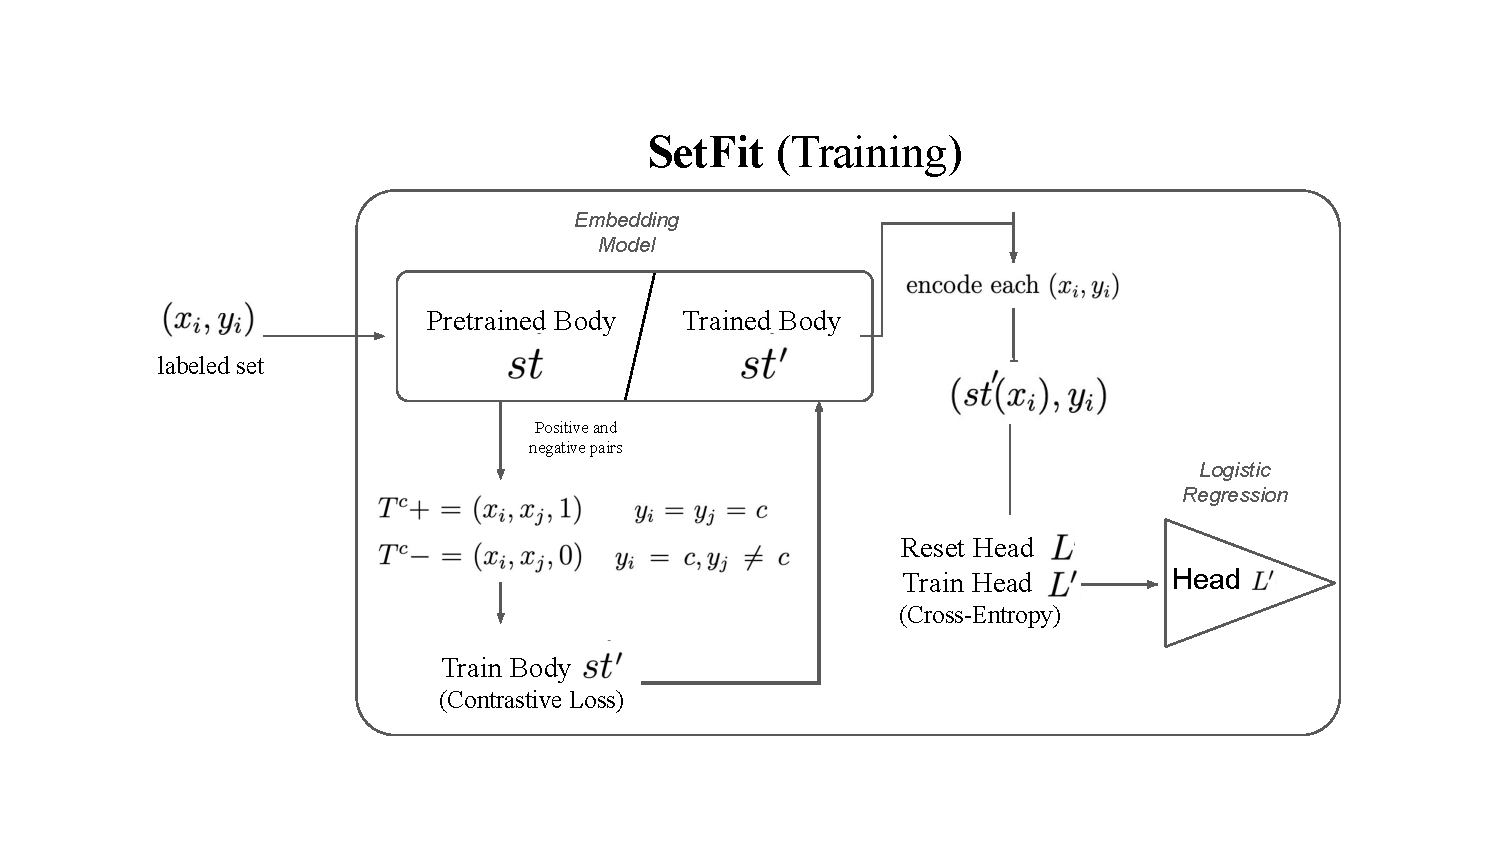
\includegraphics[width=1.1\textwidth]{figuras/Untitled presentation.pdf}}
    \caption[Diagram of the SetFit algorithm]{Diagram of the SetFit algorithm. Initially, it receives a labeled dataset $D$ with $N$ documents. It builds positive and negative pairs (which means pairs of the same class and of different classes, respectively) and performs contrastive learning to fine-tune a pretrained Sentence Transform $st$ (``body"). Then, the algorithm uses the trained $st'$ to encode documents into embeddings $st'(x_i)$ and compose pairs $(st'(x_i), y_i)$ to train a Logistic Regression ``head" with cross-entropy.}
    \label{fig:setfit}
\end{figure}

Complementary research improves general-purpose embeddings \cite{muennighoff2023mteb,lee2024nvembed,duquenne2023sonar}. Our work extends SetFit’s efficiency to the zero-shot regime by replacing manual labels with pseudo-labels derived from unlabeled corpora, coupled with diversity-aware selection.

\section{Informed Data Selection and Annotation Efficiency}
\label{sec:data_selection}

When minimal human supervision is possible, which data to annotate matters as much as how many. Crowdsourcing frequently introduces inconsistency and bias \cite{nowak2010reliable,hovy2013learning,karpinska2021perils,zhang2023needle,hsueh2009data}. Random sampling is inefficient and favors majority classes in imbalanced settings \cite{He2009LearningFI,Elkan2001,beijbom2014random}. Active learning highlights balancing uncertainty, diversity, and density \cite{ren2021survey,zhu2010,kee2018,sener2018active}. Our informed data selection work \cite{alcoforado2024random} uses diversity to build small, effective few-shot sets, which complements the zero-shot pipeline of \texttt{ZeroBERTo-2} when a small annotation budget is available. Related efforts also study informed selection for adversarial training \cite{mendoncca2022adversarial} and, at larger scales, data curation for PLMs \cite{albalak2024a,qin2025unleashing,doremi,liu2025regmix,penedo2024fineweb}.

\section{Multilinguality and Long-Document Considerations}
\label{sec:multilingual_long}

Multilingual PLMs (e.g., mBERT \cite{multilingualbert}, XLM-R \cite{DBLP:journals/corr/abs-1911-02116}) support cross-lingual transfer \cite{conneau2020unsupervised}, but zero-shot transfer has practical limits \cite{lauscher-etal-2020-zero}. For Brazilian Portuguese, there is still a lack of resources in NLP: BERTimbau \cite{souza2020bertimbau}, benchmarks like ASSIN and ASSIN2 (which evaluate model competency on Semantic Similarity and Textual Entailment) \cite{fonseca2016assin,real2020assin} and CSTNews (for news classification) \cite{cardoso2011cstnews} underscore the need for robust, resource-efficient methods beyond English. Long documents remain challenging, but compression via topics or clusters is an effective alternative to expensive long-context architectures for zero-shot classification \cite{alcoforado2022zeroberto}.

\section{Summary and Gap}
\label{sec:review_summary}

To summarize, zero-shot text classification typically relies on either large entailment-based PLMs or LLMs (strong performance, weak usability) or efficient few-shot methods (small models, but some labels needed). Self-training reduces label requirements but needs careful pseudo-label curation. Topic modeling and clustering provide a principled way to compress long inputs, but there is still not enough research on different types of clustering or in applying clustering to different steps of zero-shot pipelines. \texttt{ZeroBERTo-2} fills this gap by combining (i) unlabeled-data self-training with compact Sentence Transformers, (ii) diversity-aware pseudo-label selection — yielding a practical, lightweight zero-shot pipeline that remains competitive with larger models.

\chapter{Proposed Algorithm}
\label{chapter_zeroberto2}

This chapter presents \texttt{ZeroBERTo-2}, a low-resource-by-design pipeline for zero-shot text classification that learns exclusively from unlabeled data and runs on consumer hardware. The method builds upon compact Sentence Transformers and adapts SetFit’s contrastive fine-tuning \cite{setfit} to a self-training regime: starting from label names as textual anchors, the model computes an initial, purely unsupervised “First-Shot” score, selects high-quality and diverse pseudo-labeled data, and iteratively refines a small encoder–classifier stack. Unlike entailment-based zero-shot approaches \cite{yin2019benchmarking}, our method does not require large PLMs, prompts, or labeled validation data. 

However, a central challenge we explicitly address is label-free early stopping: without ground-truth validation, self-training may diverge over iterations and degrade performance, with sensitivity to dataset-dependent hyperparameters. We document this phenomenon and outline unsupervised stopping signals to be studied throughout this research.

Section~\ref{sec:setup} formalizes the problem and assumptions. Section~\ref{sec:pipeline} overviews the pipeline proposed for \texttt{ZeroBERTo-2} and provides pseudo-code. Sections~\ref{sec:firstshot}–\ref{sec:inference} detail each component: First-Shot scoring, data selection heuristics, contrastive self-training of the encoder and supervised training of the head, and inference. Section~\ref{sec:stopping} discusses label-free early stopping and model selection. Section~\ref{sec:hparams} summarizes practical hyperparameters.

\section{Problem Setup and Assumptions}
\label{sec:setup}

% Let $U=\{x_i\}_{i=1}^{N}$ be an unlabeled corpus and $C=\{c_1,\dots,c_m\}$ a set of target classes, specified only by their names or short natural-language descriptions. We assume an encoder (pretrained Sentence Transformer) $st_0$ and a lightweight classification head $L$ (logistic regression). The encoder $st_0$ maps texts into a k-dimensional embedding space $\phi: \mathcal{X}\to\mathbb{R}^k$. \texttt{ZeroBERTo-2} must learn a classifier $Z(x)=L(st(x))$ without any labeled examples, by iteratively: (i) producing initial scores from label names (First-Shot), (ii) selecting pseudo-labeled training data with an unsupervised heuristic, (iii) refining the encoder via contrastive learning and training the head on pseudo-labels.
% The method operates entirely without human annotation, large GPUs, or prompts, and targets practical deployment on consumer hardware.

Let $U = \{x_1, x_2, ..., x_{N}\}$ denote the unlabeled text corpus, where each $x_i$ corresponds to a document, e.g., $x_1 =$ ``The stock market rose today'', $x_2 =$ ``Brazil won the football match'', etc. We use $|U| = N$ to indicate the number of unlabeled documents. Let $C = \{c_1, ..., c_m\}$ represent the set of target classes, each described by a name or short phrase. For instance, for a news classification task, $C = \{\text{‘sports’}, \text{‘business’}, \text{‘world’}, \text{‘technology’}\}$, so $c_1 = $ ``sports'', $c_2 = $ ``business'', etc. We use $|C| = m$ to indicate the total number of classes. Both $N$ and $m$ are constant across self-training iterations. We use $n$ to indicate the number of samples per class to be selected for each self-training step, and $n_t$ for the chosen $n$ at iteration $t$.

We assume access to a pretrained Sentence Transformer encoder, denoted as $st_0$, that maps any input text (document or label name) into a $d$-dimensional embedding vector. This mapping is expressed as $\phi := st_0: \mathcal{X} \rightarrow \mathbb{R}^d$, where $\phi(x_i) = \mathbf{v}_i$ and $\phi(c_j) = \mathbf{\ell}_j$. We also assume access to a randomly initialized ``head'' (in our case, a Logistic Regression algorithm) $L$, updated to $L'$ for every self-training iteration.

Our objective is to learn a classifier $Z(x) = L(st(x))$ entirely without human-labeled data, by (i) using label names/descriptions as semantic anchors, (ii) producing initial class compatibility scores (First-Shot), (iii) selecting a set of pseudo-labeled training samples through unsupervised data selection, and (iv) iteratively refining a small encoder-classifier stack.

\section{Pipeline Overview}
\label{sec:pipeline}

% Algorithm~\ref{alg:zeroberto2} summarizes \texttt{ZeroBERTo-2}. Starting from $st_0$ and label names, the First-Shot step (FS) computes class probabilities via cosine similarity and softmax. A data selector $sel_H$ (heuristic $H$) chooses a balanced, diverse pseudo-labeled subset per class. The encoder is refined contrastively on pseudo-labels (as in SetFit \cite{setfit}), and the head is trained supervisedly on the refined embeddings. The process may iterate until a stopping rule $S$ triggers. In the absence of labels, $S$ is currently instantiated by fixed iteration budgets or unsupervised signals (Section\ref{sec:stopping}).

Figure~\ref{fig:zeroberto} sketches the ZeroBERTo 2.0 pipeline, which comprises four main modules: 
\textbf{A) Embedding Initialization:} Embed label names or short descriptions (e.g., $c_1=$ ``sports'') using a pretrained embedding model $st_0$, obtaining $\{\mathbf{\ell}_1, ..., \mathbf{\ell}_m\}$ and embed all input documents $x_i$ to obtain $\mathbf{v}_i = st_0(x_i)$.
\\ \textbf{B) First-Shot Scoring (FS):} Score each $(x_i, c_j)$ pair by cosine similarity, $\text{sim}(\mathbf{v}_i, \mathbf{\ell}_j)$; produce class probabilities via softmax.
\\ \textbf{C) Data Selection Heuristics:} Select $n$ pseudo-labeled documents per class, forming a balanced training subset $\mathcal{S}_t$ using heuristics that balance confidence and embedding diversity.
\\ \textbf{D) Self-Training Loop: }(i) Train $st'$ contrastively on selected pseudo-labeled pairs; (ii) train a logistic regression head $L'$ on the pseudo-labels and new embeddings; (iii) optionally, repeat steps C) and D), until a stopping criterion is met.


\begin{figure}[ht]
    \centerline{
    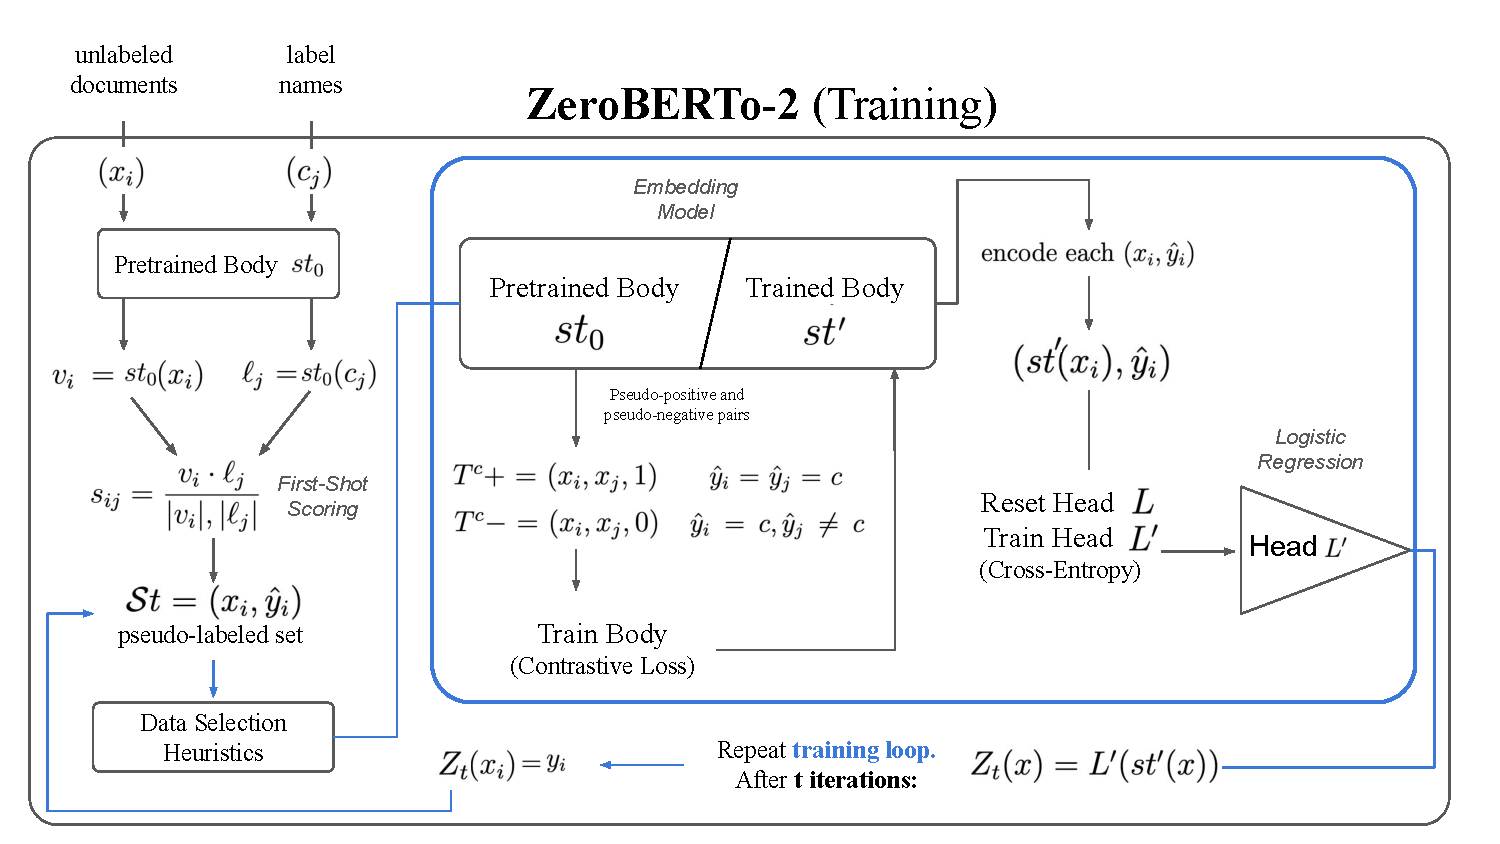
\includegraphics[width=\textwidth]{figuras/zeroberto-arch.pdf}}
    \caption[Diagram of the \texttt{ZeroBERTo-2}]{Diagram of the \texttt{ZeroBERTo-2}. Initially, it receives only an unlabeled corpus $U = x_i$  with $N$ documents and a set of classes $C$ represented by their label names $c_j$ and executes a first labeling step (First-Shot scoring) with pretrained $st_0$ to obtain a pseudo-labeled set $St = (x_i,\hat{y}_i)$. Then, an informed data selection step is executed to select the most informative and diverse examples for the self-training loop. It then iteratively trains a classifier until a stopping criteria is met, re-executing both pseudo-labeling and data selection steps.}
    \label{fig:zeroberto}
\end{figure}

% xxx adicionar diagrama de inferencia


%xxx[Insert pipeline figure here: each module as a block, with example inputs/outputs: $x_1$ ("Brazil won...") → $v_1$ → scores $\mathbf{p}_1$, etc.]

The pseudo-code for the overall iterative optimization is given in Algorithm~\ref{alg:zeroberto2}.

\begin{algorithm}[h]
\SetAlgoLined
\KwData{
Unlabeled corpus $U=\{x_i\}$; class set $C=\{c_j\}$ (names or descriptions);\newline
Pretrained Sentence Transformer $st_0$; head $L$ (logistic regression);\newline
Selector $sel_H$ with heuristic $H$; samples per class $n$; iterations $T$ or stopping rule $S$;\newline
Contrastive pairs per class $R$; batch/optimizer hyperparameters.}
\KwResult{Trained model $Z=L'(st')$ and pseudo-labeled set $\mathcal{S}$}
Initialize $st \leftarrow st_0$; initialize $L$ randomly;
Compute label embeddings ${\ell_j=st(c_j)}_{j=1}^m$;
\For{$t=1$ \KwTo $T$}{
$\mathbf{p}i = \emptyset$\\
\tcp{\textit{First-Shot scoring (FS)}}
\ForEach{$x_i \in U$}{
$v_i \leftarrow st(x_i)$; $s_{ij}\leftarrow \cos(v_i,\ell_j)$ for all $c_j\in C$;\\
$p_{ij}\leftarrow \text{softmax}_j(s_{ij})$; $\mathbf{p}i = \mathbf{p}i \cup \{p_{ij}\}$
}
\tcp{\textit{Pseudo-label selection}}
$\mathcal{S}t \leftarrow sel_H\big({(x_i,\mathbf{p}i,v_i)}_{i=1}^N,n\big)$;

\tcp{\textit{Contrastive encoder refinement (pseudo-labels)}}
Build positive/negative pairs $T_{enc}$ from $\mathcal{S}t$ (Section~\ref{sec:selftraining});\\
Update $st \leftarrow \text{ContrastiveTrain}(st,T_{enc})$;

\tcp{\textit{Head training on refined embeddings}}
Encode $\mathcal{S}t$ with $st$ to form $T_{head}={(st(x),\hat{y})}$;\\
Reset $L$ and train $L \leftarrow \text{Train}(L,T_{head})$;

\tcp{\textit{Optional: evaluate unsupervised stopping signals}}
\If{$S$ triggers}{break}
}
Return $Z(x)=L(st(x))$ and $\mathcal{S}^=\bigcup_{t}\mathcal{S}_t$;
\caption{\texttt{ZeroBERTo-2}: Unlabeled-only zero-shot self-training}
\label{alg:zeroberto2}
\end{algorithm}

\section{First-Shot Scoring}
\label{sec:firstshot}

Let $v_i=st(x_i) \in \mathbb{R}^d$ be the document $x_i$ and its respective embedding $v_i$, with $i = 1 \dots N$,  and $\ell_j=st(c_j)\in \mathbb{R}^d$, with $j = 1 \dots m$ the label embedding computed from the label name or description. We define scores and probabilities by
\begin{equation}
s_{ij} = \frac{v_i \cdot \ell_j}{|v_i|,|\ell_j|},
\label{eq:firstshotscores}
\end{equation}

\begin{equation}
p_{ij} = \frac{\exp(s_{ij}/\tau)}{\sum_{k=1}^{m}\exp(s_{ik}/\tau)},
\label{eq:firstshotsprobs}
\end{equation}
where $\tau>0$ is an optional temperature that we introduce to the traditional softmax formula. The First-Shot (FS) probabilities $\mathbf{p}i=(p_{i1},\dots,p_{im})$ serve as inputs to the data selector. This simple, label-name–driven compatibility is a standard and efficient zero-shot mechanism \cite{yin2019benchmarking}.

\section{Data Selection Heuristics}
\label{sec:selection}

Given ${(x_i,\mathbf{p}_i,v_i)}$, the selector $sel_H$ chooses $n$ pseudo-labeled samples per class to form $\mathcal{S}t = \{(x,\hat{y})\}$, with $\hat{y}=\arg\max_j p{ij}$. We use two generic, unsupervised heuristics:

\textbf{1) $top~n$ per class:} select the $top~n$ highest-confidence samples per predicted class, enforcing per-class balance. For instance, if $n = 8$ samples per class, and $m = 4$ classes, $top~n$ will select, for each 4 classes, the 8 highest scores as calculated in the previous labeling step (which can be First-Shot scoring with cosine similarity or the inference of a trained $Z_t$ after $t$ self-training loops).

\textbf{2) Intra-class clustering:} for each predicted class, cluster the embeddings ${v_i}$ and pick high-confidence representatives from distinct clusters to maximize diversity. Algorithm~\ref{alg:intra} gives a generic procedure; any clustering (e.g., k-means++, HDBSCAN) can be adopted. This heuristic mitigates mode collapse and encourages coverage of sub-modes within each class.

\begin{algorithm}[h]
\caption{Data Selection via Intra-class Clustering}
\label{alg:intra}
\SetKwInOut{Input}{inputs}
\SetKwInOut{Output}{output}
\Input{Embeddings $V={v_i}$; probability matrix $P \in \mathbb{R}^{|V|\times m}$; samples per label $n$}
\Output{Selected indices per label $\mathcal{I}={\mathcal{I}\ell}{\ell=1}^m$}
\For{$\ell=1$ \KwTo $m$}{
$V_\ell \leftarrow {v_i:\arg\max_j P_{ij}=\ell}$; $P_\ell \leftarrow {P_{i\ell}: \arg\max_j P_{ij}=\ell}$;\\
$\mathcal{C}\ell \leftarrow \textbf{Clustering}(V\ell)$ \tcp*{\textit{map clusters to member indices}}
$\mathcal{I}\ell \leftarrow \emptyset$;\\
\While{$|\mathcal{I}\ell|<n$}{
\ForEach{cluster $c\in \mathcal{C}\ell$}{
$i^\star \leftarrow \arg\max{i\in c} P_{i\ell}$;
Remove $i^\star$ from $c$; $\mathcal{I}\ell \leftarrow \mathcal{I}\ell \cup {i^\star}$;
\lIf{$|\mathcal{I}_\ell|\ge n$}{break}
}
}
}
\KwRet{$\mathcal{I}$}
\end{algorithm}

Both heuristics accept simple add-ons: (i) a confidence floor on $p_{ij}$, (ii) temperature scaling in Eq. \ref{eq:firstshotsprobs}, (iii) maximum-per-cluster caps, and (iv) class-balancing. These controls, although label-free, are dataset-dependent; Section \ref{sec:stopping} discusses their connection to early stopping.

\section{Self-Training: Encoder Contrastive Refinement and Head Training}
\label{sec:selftraining}

At iteration $t$, let $\mathcal{S}t=\{(x_i,\hat{y}_i)\}$ be the pseudo-labeled set selected by $sel_H$. We refine the encoder $st$ via a contrastive objective in the spirit of SetFit \cite{setfit}, using cosine similarity in the embedding space. Define, for each class $c$, a set of $R$ positive pairs $T^{c}{+}=\{(x_i,x_j,1)\}$ with $\hat{y}_i=\hat{y}_j=c$, and $R$ negative pairs $T^{c}{-}=\{(x_i,x_j,0)\}$ with $\hat{y}_i=c,\hat{y}_j\neq c$. The encoder training set is $T_{enc}=\bigcup{c\in C}(T^{c}{+}\cup T^{c}{-})$ with $|T_{\text{enc}}|=2R|C|$.

We optimize $st$ to increase similarity for positive pairs and decrease for negatives (e.g., a cosine-contrastive loss). After updating $st$ to $st'$, we encode each $(x_i,\hat{y}_i)\in\mathcal{S}t$ to obtain $T_{head}=\{(st'(x_i),\hat{y}_i)\}$. The head $L$ is reset and trained with cross-entropy on $T_{head}$, yielding $L'$. The model at iteration $t$ is $Z_t(x)=L'(st'(x))$.

\section{Inference}
\label{sec:inference}

Given a trained pair $(st,L)$, the prediction for $x$ is
\begin{equation}
Z(x) = L\big(st(x)\big) = \{ z(x,c_1),\dots,z(x,c_m)\},
\end{equation}
\begin{equation}
p^Z(x,c_j) = \frac{\exp(z(x,c_j))}{\sum_k \exp(z(x,c_k))}.
\end{equation}

These probabilities can feed a subsequent selection round, enabling iterative self-training.

\section{Label-Free Early Stopping and Model Selection}
\label{sec:stopping}

In realistic zero-shot settings, there is no labeled validation to decide when to stop. We observe that self-training often improves early and then diverges, degrading performance in later iterations.
The best iteration and stability are sensitive to hyperparameters (e.g., $n$, $R$, clustering granularity, temperature), and the “best” configuration varies across datasets.
To make zero-shot self-training reliably usable, we frame label-free early stopping as a central open problem and study unsupervised signals that can trigger $S$ in Algorithm~\ref{alg:zeroberto2}. 

Because \texttt{ZeroBERTo-2} is a lightweight model, it is possible to reinstantiate the model many times during a single training run. Therefore, our architecture is flexible, for which there are many options of candidate signals for early stopping, which include:\\
i) \textbf{Confidence trends:} mean/max confidence, calibration proxies, or margin statistics; saturation or sudden drifts may indicate overfitting on self-confirming pseudo-labels. \\
ii) \textbf{Entropy dynamics:} monitoring the entropy $H(\mathbf{p})$ over $U$; premature entropy collapse can correlate with degraded generalization. \\
iii) \textbf{Cross-iteration agreement:} stability of predictions between $Z_{t-1}$ and $Z_t$; sharp increases in disagreement after peaking may signal divergence. \\
iv) \textbf{Diversity/compactness: }cluster separation and within-class dispersion (e.g., silhouette) on embeddings; excessive compaction can indicate mode collapse. \\
v) \textbf{Split-then-compare:} unsupervised holdout of $U$ to track the above signals on disjoint subsets.

The present work documents the phenomenon but does not yet compare these signals, developing a principled, robust stopping rule without labels is still an ongoing work and concluding goal of this research.

\section{Hyperparameters and Practical Settings}
\label{sec:hparams}

\texttt{ZeroBERTo-2} is designed for small backbones (e.g., compact Sentence Transformers) and modest hardware. Key hyperparameters are:\\
\textbf{i) Selection:} samples per class $n$; temperature $\tau$; clustering method and number of clusters or density parameters; per-cluster caps.\\
\textbf{ii) Contrastive refinement:} pairs per class $R$; batch size; optimizer and learning rate; iterations $T$ or stopping rule $S$.\\
\textbf{iii) Head: }logistic regression (or shallow MLP) with cross-entropy; reinitialized each iteration.

In practice, different datasets favor different settings; currently, consistent peak performance requires per-dataset hyperparameter tuning to avoid late-iteration collapse. This dependence reinforces the need for label-free model selection criteria (Section~\ref{sec:stopping}). Despite this limitation, the pipeline often matches or surpasses larger, more complex zero-shot baselines at its best iteration, while remaining feasible on consumer hardware—fulfilling the low-resource-by-design objective.

\medskip
Overall, \texttt{ZeroBERTo-2} operationalizes unlabeled-only, small-model zero-shot classification by combining label-name–driven First-Shot scoring, diversity-aware pseudo-label selection, and contrastive self-training. The remaining challenge lies in principled, label-free early stopping to guarantee robust performance across datasets.


\chapter{Experimental Setup}
\label{chapter_test}

This chapter details the datasets, baselines, evaluation metrics, protocols, and implementation choices used to assess \texttt{ZeroBERTo-2}. Our goal is to compare a small-model, unlabeled-only zero-shot pipeline both against strong zero-shot baselines and efficient few-shot methods, while explicitly measuring accuracy under low-resource constraints.

Instead of beginning by describing the data, instead we choose which baselines are going to be considered in the comparison to ZeroBERTo. We then present the datasets and our evaluation protocol. Finally, we specify implementation details and hyperparameters applied to our experiments.

\section{Baselines}
\label{sec:baselines}



We compare \texttt{ZeroBERTo-2} against two families of baselines: first, we test it against two different few-shot methods: fine-tuning of XLM-R and the traditional pipeline of SetFit. Then, we compare \texttt{ZeroBERTo-2} to chosen zero-shot pipelines.

\subsection{Few-Shot Learning}

\textbf{i) Fine-Tuning of XLM-R (Conneau et al.,
2020):}
We fine-tune the XLM-Roberta-large , a pre-trained encoder-based Language Model, following conventional fine-tuning procedures for Sequence Classification. The training process spans 30 epochs with a learning rate of $2 \times 10^{-5}$.

\textbf{ii) SetFit (Tunstall et al.,
2022):} We compare \texttt{ZeroBERTo-2} to the traditional Sentence
Transform Fine-Tuning (SetFit) pipeline, an efficient approach for few-shot
learning in encoder-based models. SetFit dynamically generates training pairs from
annotated data and leverages contrastive loss for training the model on the classification task. As the base model, we use \texttt{paraphrase-multilingual-mpnet-base-v2}.
%%%%a

\subsection{Zero-Shot Learning}

\textbf{i) PESCO: Prompt-enhanced Self Contrastive Learning for Zero-shot Text Classification \cite{wang2023pesco}:}
This is a self-training framework for zero-shot classification that uses prompts to enhance performance, which \texttt{ZeroBERTo-2} does not need. The self-training consists of two iterative steps, pseudo-label prediction and model update. This method is referred to as \texttt{PESCO} in tables \ref{tab:zs1} and \ref{tab:zs2}. 

% \textbf{i) Prompt-based Zero-Shot Classification (Wei et al., 2022):}
% This approach leverages large language models (LLMs) by converting classification tasks into natural language prompts, allowing the model to infer the correct label without any task-specific training. The authors evaluate their method on benchmarks including AG News, DBPedia, Yelp, Amazon, and TREC.

\textbf{ii) Zero-Shot Text Classification with Self-Training \cite{gera2022zero}:}
This paper introduces a plug-and-play self-training method for zero-shot text classification. It leverages large pre-trained language models fine-tuned on natural language inference datasets. The approach involves iteratively fine-tuning the model on its most confident predictions using only class names and unlabeled data, without requiring domain expertise. This method is referred to as \texttt{ZERO\_001} in tables \ref{tab:zs1} and \ref{tab:zs2}. 

\textbf{iii) Zero-Shot Text Classification via Self-Supervised Tuning \cite{liu2023zero}:}
This work proposes a self-supervised tuning paradigm for zero-shot text classification. Instead of relying on prompt engineering or large-scale annotated data, it introduces a novel learning objective called "first sentence prediction," which trains the model to predict the first sentence of a paragraph based on the rest. This approach addresses the gap between unlabeled data and classification tasks, achieving state-of-the-art results on 7 out of 10 tasks while being less sensitive to prompt design, but still requires some form of prompting which \texttt{ZeroBERTo-2} does not. This method is referred to as \texttt{ZERO\_002} in tables \ref{tab:zs1} and \ref{tab:zs2}. 

% \textbf{ii) Z-STAR: Zero-Shot Text Classification with Self-Training and Label Augmentation (Zhao et al., 2023):}
% Z-STAR combines self-training with label augmentation, using pseudo-labels generated by a teacher model to iteratively improve a student model in a zero-shot setting. The method is evaluated on datasets such as AG News, Yahoo! Answers, and DBPedia.

% \textbf{iii) ZEST: Zero-Shot Learning from Text Descriptions (Huang et al., 2023):}
% ZEST introduces a method that aligns textual descriptions of classes with input text representations, enabling zero-shot classification by matching input samples to class descriptions. The authors conduct experiments on datasets including AG News, Yahoo! Answers, and DBPedia.


% \textbf{iv) ZS-Few: Zero-Shot to Few-Shot Text Classification with Weak Supervision (Zhang et al., 2023):}
% ZS-Few proposes a weakly supervised framework that transitions from zero-shot to few-shot learning by leveraging weak supervision signals, such as noisy labels or external knowledge. The framework is evaluated on AG News, Yahoo! Answers, and DBPedia datasets.

% We need to explain each of these methods in max 2 sentences:

% https://arxiv.org/pdf/2210.17541
% https://arxiv.org/abs/2305.11442
% https://arxiv.org/pdf/2305.13723.pdf
% https://arxiv.org/pdf/2305.14963.pdf

% Sentence-Transformer cosine baseline: all-mpnet-base-v2 (hf: sentence-transformers/all-mpnet-base-v2). Classify by cosine similarity between document and label embeddings with softmax over labels.


% Optional multilingual baseline: paraphrase-multilingual-MiniLM-L12-v2 for non-English datasets.


\section{Datasets}
\label{sec:datasets}

We select classification datasets that cover diverse domains and difficulty levels, including news/topic categorization, sentiment/emotion, and intent detection. In order to adequately compare \texttt{ZeroBERTo-2} to chosen baselines, we include all 15 datasets used by these baselines. When available, we rely on official splits; otherwise, we report the splitting strategy. We use the test splits for evaluation only. For zero-shot training, we only access unlabeled text from the training split (labels are discarded). 

Table~\ref{tab:datasets} summarizes the datasets. For each dataset, we report domain, number of classes, average document length (tokens), train/test sizes, and language.

\begin{itemize}

\item \textbf{AG News (AGN):} Contains news articles categorized into four classes: World, Sports, Business, and Science/Technology.
\item \textbf{20 Newsgroups (20NG):} A collection of approximately 20,000 newsgroup documents, organized into 20 categories.
\item \textbf{BBC News:} Comprises news articles from the BBC, divided into five categories: Business, Entertainment, Politics, Sport, and Tech.
\item \textbf{DBpedia}: Derived from Wikipedia, this dataset includes 14 non-overlapping classes such as Company, Educational Institution, Artist, Athlete, and more.
\item \textbf{Amazon Reviews (AmazonReviewPolarity)}: Consists of product reviews labeled with positive or negative sentiment.
\item \textbf{Amazon Reviews (AmazonReviewFull)}: Contains product reviews with ratings from 1 to 5 stars.
\item \textbf{EmotionLines}: Focuses on detecting emotions in conversations, with seven emotion categories.
\item \textbf{Customer Reviews (CR)}: A dataset of customer reviews used for sentiment analysis tasks.
\item \textbf{Enron Spam (enrspam)}: A collection of emails used for spam detection, containing both spam and ham (non-spam) emails.
\item \textbf{Stanford Sentiment Treebank (SST-5)}: Provides fine-grained sentiment labels (very negative to very positive) for movie reviews.
\item \textbf{IMDb Reviews}: Contains 50,000 movie reviews, evenly split between positive and negative sentiments.
\item \textbf{Yahoo! Answers}: Comprises questions and answers from Yahoo! Answers, categorized into ten classes.
\item \textbf{Stanford Sentiment Treebank (SST-2)}: A binary version of SST-5, with positive and negative sentiment labels.
\item \textbf{Yelp Reviews (Yelp-5)}: Contains Yelp reviews with ratings from 1 to 5 stars.
\item \textbf{Movie Reviews (MR)}: A dataset of movie reviews used for binary sentiment classification.

\end{itemize}


\begin{table}[]
\caption{Datasets used to assess \texttt{ZeroBERTo-2} performance.}
\label{tab:datasets}
\vspace{0.5cm}

\resizebox{0.95\textwidth}{!}{%
\begin{tabular}{ccccc}
Dataset Name                        & Domain               & Number of Classes & Training Size & Testing Size \\
AG News (AGN)                       & News Articles        & 4                 & 30000           & 1900         \\
20 Newsgroups (20NG)                & Newsgroup Messages   & 20                & 11,314        & 7,532        \\
BBC News                            & News Articles        & 5                 & 1,998         & 1            \\
DBpedia                             & Encyclopedia Entries & 14                & 560           & 70           \\
Amazon Reviews (Polarity)           & Product Reviews      & 2                 & 3,600,000     & 400          \\
Amazon Reviews (Full)               & Product Reviews      & 5                 & 3,000,000     & 650          \\
EmotionLines                        & Conversations        & 7                 & 15            & 2            \\
Customer Reviews (CR)               & Product Reviews      & 2                 & 3,775         & 1,125        \\
Enron Spam (enrspam)                & Emails               & 2                 & 33,716        & 16,555       \\
Stanford Sentiment Treebank (SST-5) & Movie Reviews        & 5                 & 8,544         & 2,21         \\
IMDb Reviews                        & Movie Reviews        & 2                 & 25            & 25           \\
Yahoo! Answers                      & Q\&A Platform        & 10                & 1,400,000     & 60           \\
Stanford Sentiment Treebank (SST-2) & Movie Reviews        & 2                 & 67,349        & 872          \\
Yelp Reviews (Yelp-5)               & Business Reviews     & 5                 & 650           & 50           \\
Movie Reviews (MR)                  & Movie Reviews        & 2                 & 8,662         & 2           
\end{tabular}

}
\end{table}
% \begin{table*}[htbp]
% \centering
% \caption{Datasets used in our experiments.}
% \label{tab:datasets}
% \setlength{\tabcolsep}{6pt}
% \renewcommand{\arraystretch}{1.1}
% \begin{tabularx}{\textwidth}{l l c c r r l}
% \toprule
% Dataset & Domain & Number of Classes & Avg. Doc Length (tokens) & Train Size & Test Size & Language \
% \midrule
% AG News (AGN) & News Articles & 4 & $\sim$200 & 120{,}000 & 7{,}600 & English \
% 20 Newsgroups (20NG) & News Articles & 20 & $\sim$200 & 11{,}314 & 7{,}532 & English \
% BBC News & News Articles & 5 & $\sim$200 & 2{,}225 & 570 & English \
% DBpedia & Wikipedia Articles & 14 & $\sim$200 & 560{,}000 & 70{,}000 & English \
% Amazon Reviews (AmazonReviewPolarity) & Product Reviews & 2 & $\sim$200 & 3{,}600{,}000 & 400{,}000 & English \
% Amazon Reviews (AmazonReviewFull) & Product Reviews & 5 & $\sim$200 & 3{,}000{,}000 & 650{,}000 & English \
% EmotionLines & Conversations & 7 & $\sim$20 & 29{,}245 & N/A & English \
% Customer Reviews (CR) & Product Reviews & 2 & $\sim$20 & 3{,}775 & N/A & English \
% Enron Spam (enrspam) & Emails & 2 & $\sim$200 & 33{,}717 & 16{,}555 & English \
% Stanford Sentiment Treebank (SST-5) & Movie Reviews & 5 & $\sim$20 & 8{,}544 & 2{,}210 & English \
% IMDb Reviews & Movie Reviews & 2 & $\sim$200 & 25{,}000 & 25{,}000 & English \
% Yahoo! Answers & Question Answers & 10 & $\sim$200 & 1{,}400{,}000 & 60{,}000 & English \
% Stanford Sentiment Treebank (SST-2) & Movie Reviews & 2 & $\sim$20 & 6{,}920 & 1{,}821 & English \
% Yelp Reviews (Yelp-5) & Product Reviews & 5 & $\sim$200 & 650{,}000 & 50{,}000 & English \
% Movie Reviews (MR) & Movie Reviews & 2 & $\sim$20 & 10{,}662 & N/A & English \
% \bottomrule
% \end{tabularx}
% \end{table*}

% \subsection{Label Names and Verbalizations}
% \label{sec:labels}

% \texttt{ZeroBERTo-2} assumes only label names or short natural-language descriptions. For each dataset:

% If canonical label names exist (e.g., joy, sadness), we use them directly.
% If names are ambiguous, we add 1–3 short verbalizations per label (e.g., “topic: world news”, “financial/business news”).
% For multilingual datasets, label names are provided in the dataset language; if unavailable, we use English names and rely on multilingual encoders for cross-lingual alignment.
% For entailment-based baselines, we adopt standard hypothesis templates per label (Section~\ref{sec:baselines}), keeping templates minimal and consistent across methods.


\section{Evaluation Protocol}
\label{sec:protocol}

\textbf{Zero-Shot Constraint}: 
No task-specific labels are used for the training of the model. \texttt{ZeroBERTo-2} accesses only unlabeled documents from the train split and the label names.


\textbf{Metrics}: Every baseline chooses Accuracy as the primary metric for reporting performance, which we also adopt in order to keep a fair comparison. We also take into account the \textbf{imbalance} of classes as a variable, so we also report both Macro and Micro F1-scores. 
We report the accuracy of a single ZeroBERTo iteration in all cases since our model is deterministic. 


\section{Implementation Details}
\label{sec:implementation}



Since our goal is to build a model that can run on consumer hardware, all our experiments are conducted with Google Colab Free: GPUs are NVIDIA V100 16GB or T4 16GB; CPU is Intel Xeon-class.
All runs fit within 12 GB VRAM. Batch size was kept constant at 8.

The software kit we used is also very traditional within our context of low-resource NLP. Our repository is in Python, with libraries PyTorch, Transformers, sentence-transformers, scikit-learn, HDBSCAN (our choice for clustering algorithm), numpy/scipy.


\section{Stopping Signals without Labels}
\label{sec:stopping_protocol}

This part of the research is still ongoing. We intend to design an effective set of unsupervised signals that we can measure after each iteration. These signals should indicate whether our model is likely overfitting, underfitting or has gone through mode colapse (ie. when the model produces less variety of labels than expected). 

For the experiments already conducted, the stopping signal used was a hard-stop set by the hyperparameter configuration. This hyperparameter, however, is very sensible to the choice of dataset.

% Confidence dynamics: saturation of mean confidence or sudden increases in max–mean gap.
% Entropy: average predictive entropy over the unlabeled pool; early collapse triggers a stop.
% Cross-iteration agreement: Jaccard or Cohen’s κ between successive predictions; a sharp increase in disagreement after prior improvement signals divergence.
% Embedding compactness: silhouette score within predicted classes; excessive compaction after gains indicates overfitting. In all cases, we impose a minimum of one full iteration before stopping. When no signal triggers, we stop at the budget T.

\chapter{Results}
\label{chapter_result}

In this chapter, we show the results of the tests conducted until now.

\section{Few-Shot Pipelines}

\textbf{\texttt{ZeroBERTo-2} delivers a strong performance} when compared to other few-shot methods. Table \ref{fs-results} shows comparative results (Accuracy) to both XLM-R fine-tuning and SetFit, bringing mean and standard deviation for the baselines. We see that \texttt{ZeroBERTo-2} outperforms XLM-R for $n = 8$, while matching SetFit performance. For $n = 64$, SetFit is a better choice for most datasets, but \texttt{ZeroBERTo-2} still keeps competitive with XLM-R. We present fully-supervised training results of XLM-R just as a reference, as it is unfair to compare a zero-shot model to a fully supervised one.

An important comment to be made is that both XLM-R and SetFit are stochastic algorithms, as selection of the initial few-shot dataset is a random process. \texttt{ZeroBERTo-2}, on the other hand, selects the initial data in a deterministic way. Thus, \textbf{achieving a performance slightly superior to the mean accuracy} of these baselines is already a \textbf{superior result}.

% Please add the following required packages to your document preamble:
% \usepackage{graphicx}
\begin{table}[]
\caption{Results of comparing to few-shot models.}
\resizebox{\textwidth}{!}{
\begin{tabular}{|ccllllll|}
\hline \hline
                      \texttt{n}     &    Model    & \textbf{agn}        & \textbf{amz\_cf}     & \textbf{emotion}    & \textbf{cr}         & \textbf{enrspam}    & \textbf{sst5}       \\ \cline{2-9} \hline
\multicolumn{1}{|c}{\texttt{0}} & \texttt{ZeroBERTo}_{mpnet}         & $83.55$      & \textbf{x}  & $51.3$       & $91.48$      & \textbf{x} & $43.84$      \\ 
\cline{2-9} \hline
\multicolumn{1}{|c}{\texttt{8}}  & \textsc{FineTune}_{roberta}& $ 81.7_{3.8} $ & $ 9.2_{4.9} $   & $ 28.7_{6.8} $  & $ 58.8_{6.3} $ & $ 85.0_{6.0} $ & $ 33.5_{2.1} $ \\
\multicolumn{1}{|c}{}      & \textsc{SetFit}_{mpnet}       & $ 82.9_{2.8} $ & $ 40.3_{11.8} $ & $ 48.8_{4.5} $ & $ 88.5_{1.9} $ & $ 90.1_{3.4} $ & $ 43.6_{3.0} $ \\ \cline{2-9} \hline
\multicolumn{1}{|c}{\texttt{64}} &\textsc{ FineTune}_{roberta} & $ 88.4_{0.9} $ & $ 52.8_{12.1} $ & $ 65.0_{17.2} $ & $ 88.9_{1.9} $ & $ 95.9_{0.8} $ & $ 45.9_{6.9} $ \\
\multicolumn{1}{|c}{}      & \textsc{SetFit}_{mpnet}         & $ 88.0_{0.7} $ & $ 61.9_{2.9} $  & $ 76.2_{1.3} $ & $ 90.4_{0.6} $ & $ 96.1_{0.8} $ & $ 51.9_{0.6} $ \\ \cline{2-9} \hline
 \multicolumn{1}{|c}{\texttt{full}} & \textsc{FineTune}_{roberta} & $93.8$   & $80.1$        & $92.6$       & $92.4$       & $99.0$      & $59.8$ \\    
\cline{2-9} \hline
\end{tabular}
}
\label{fs-results}
\end{table}


\section{Zero-Shot Pipelines}

Tables \ref{tab:zs1} and \ref{tab:zs2} show accuracy results of ZeroBERTo compared to other zero-shot pipelines. We see that PESCO has an advantage, but a caveat to this model is that it is not easily implementable, as it uses data augmentation and multiple loss functions to guide the self-training of the model. \texttt{ZeroBERTo-2}, on the other hand, is a plug-and-play model, easy to implement as it only needs unlabeled documents and a set of classes. 

In summary, apart from PESCO, we see that no model has a clear advantage for most datasets. However, during training, we observe an interesting phenomenon. \texttt{ZeroBERTo-2} \textbf{surpasses the performance} of most other models in earlier stages of training. This is a remarkable result: because the model does not have access to any labels, it is likely that it should need more data to adequately learn the differences between classes. The sequence of training iterations contradicts this hypothesis, showing that for many datasets, our model could benefit from early stopping its training. 


\begin{table}[]
\caption{Results from zero-shot experiments.}
\begin{tabular}{|c|c|c|c|c|c|l|l|}
\hline
model    & \# params & agn   & 20ng & dbped & amz\_rvw              & \multicolumn{1}{c|}{emotion} & \multicolumn{1}{c|}{cr}    \\ \hline
\texttt{ZeroBERTo-2}  & 110 M     & 83.55 & 55   & 95.18 & \multicolumn{1}{l|}{} & \multicolumn{1}{c|}{51.3}    & \multicolumn{1}{c|}{91.48} \\ \hline
\texttt{PESCO}              & 110 M & 89.6 & \multicolumn{1}{l|}{} & 98.5 & 95.2 &  &  \\ \hline
\texttt{ZERO\_001}  & 355 M & 76.5 & 65.8                  & 92.2 & 94.3 &  &  \\ \hline
\texttt{ZERO\_002}        & 355 M & 83.7 & 56.7                  & 85.6 & 95.2 &  &  \\ \hline
\end{tabular}
\label{tab:zs1}
\end{table}

\begin{table}[t]
\caption{Results from zero-shot experiments.}

\begin{tabular}{|c|c|c|c|c|l|l|c|}
\hline
model            & \# params & sst5                  & imdb                  & yahoo & \multicolumn{1}{c|}{sst2} & \multicolumn{1}{c|}{ylp}  & mr                    \\ \hline
\texttt{ZeroBERTo-2}   & 110 M & 43.84 & 89.1 & 60.44 &  &  & 81.14 \\ \hline
\texttt{PESCO}               & 110 M     & \multicolumn{1}{l|}{} & \multicolumn{1}{l|}{} & 71.1  &                           &                           & \multicolumn{1}{l|}{} \\ \hline
\texttt{ZERO\_001} & 355 M     & \multicolumn{1}{l|}{} & 92.5                  & 59.8  &                           &                           & \multicolumn{1}{l|}{} \\ \hline
\texttt{ZERO\_002}       & 355 M     & 46.9                  & 93.0                  & 62.4  & \multicolumn{1}{c|}{90.1} & \multicolumn{1}{c|}{95.2} & 87.4                  \\ \hline
\end{tabular}
\label{tab:zs2}

\end{table}

% The first outstanding result in both datasets is that the DA  algorithm LAMBADA presented the worst result in all classifiers, using DistilBERT as a discriminator. This result may be a consequence of the low availability of data that does not allow the creation of an efficient discriminator or conditioning of the GPT-2 language model. In contrast, LAMBADA's performance improves when we use SetFit as a discriminator. This phenomenon strongly indicates that few-shot learning techniques are much more adapted to situations of a scarcity of data. In this way, the SetFit discriminator is much more successful in segregating wrong or mislabeled generations.

% The PKA algorithm performed among the best results in both datasets, especially in SemEval 2018 task 1. The performance gain concerning the other algorithms is more remarkable in all classifiers. However, the best values are with CNN, LSTM, and XLNet classifiers. This result shows that PKA has state-of-the-art competitive results compared to other DA algorithms, especially in this scenario of low data availability.

% Another interesting result is that we achieved a similar result using GPT-NEO compared to BLOOM, just putting a few-shot learning prompt with more examples (10 against 3). This performance is relevant, as we achieved similar results with a much simpler and smaller LLM, but with more operations at the prompt. Thus, we can save more computational resources by using less complex models.

% Another way to evaluate DA algorithms is by lexical diversity and semantic fidelity in the generated synthetic data. \cite{Pellicer2023} used the BLUE metrics without brevity penalty (bp) as a lexical diversity metric and the cosine similarity as a semantic meaning maintenance metric. Table \ref{Table_blue_sim} compares  LAMBADA and the proposed PKA algorithm, and shows that PKA introduces even more lexical diversity than LAMBADA, as it presented a lower BLUE. In contrast, PKA retains more semantic meaning than LAMBADA, since it has a considerably higher cosine similarity value.

\chapter{Discussion, Future Work, and Research Schedule}
\label{chapter_conc}

This chapter discusses limitations and open problems of the proposed approach, outlines concrete avenues for future work, and presents the schedule for the remaining stages of the research. The goal is to consolidate \texttt{ZeroBERTo-2} into a robust, small-model, zero-shot pipeline that is usable on consumer hardware with clear milestones.

\section{Discussion and Limitations}

\texttt{ZeroBERTo-2} advances small-model zero-shot classification by combining label-name anchoring, diversity-aware pseudo-label selection, and contrastive self-training. While results are promising, several limitations and risks remain:
\begin{itemize}
    \item \textbf{Label-free early stopping:} iterative self-training often improves early and then degrades. Without a labeled validation set, deciding when to stop is non-trivial and dataset-dependent.
    \item \textbf{Sensitivity to hyperparameters:} selection size, temperature, confidence thresholds, and clustering granularity substantially impact stability and peak performance across datasets.
    \item \textbf{Confirmation bias in pseudo-labeling: }top-confidence sampling may amplify early mistakes; diversity helps but does not eliminate this risk.
    \item \textbf{Label verbalizations: }short names/descriptions vary in specificity across datasets; ambiguous labels can hurt First-Shot alignment.
    \item \textbf{Cross-lingual and domain shift:} small encoders handle many languages reasonably well, but domain or language mismatch still degrades embedding quality.
    \item \textbf{Efficiency and deployment:} although the pipeline runs on modest hardware, additional gains (quantization, distillation) may be required for very tight budgets or on-device inference.
    \item \textbf{Evaluation coverage:} broader datasets (including PT-BR and long-form sources) and stronger baselines (e.g., recent NLI/LLM variants) are needed for a comprehensive picture.
\end{itemize}
These limitations motivate the research directions below.


\section{Future Work}
\label{sec:future_work}

In the immediate term, our priority is to complete the remaining experiments and consolidate the missing results so that \texttt{ZeroBERTo-2} is stable end-to-end and reproducible. This includes finalizing the selection–refinement loop, locking hyperparameters that consistently prevent late-iteration collapse, and documenting a default configuration that runs reliably on consumer hardware. Alongside this, we will tighten the experimental protocol (fixed seeds, dataset cards, label verbalizations, and timing/memory reporting) to ensure that the final numbers are transparent and repeatable.

The main technical objective we will pursue before closing the study is a label-free early-stopping criterion that is simple enough to adopt by default. We will compare a small set of unsupervised signals—confidence and entropy trends over the unlabeled pool, cross-iteration agreement between successive models, and basic measures of within-class compactness—and select a rule that best predicts post-peak degradation without access to validation labels. 
%If time permits, we will also test a lightweight teacher–student variant (temporal ensembling) to stabilize agreement across iterations, but our emphasis remains on a minimal policy that works within the current datasets.

In parallel, we will refine pseudo-label curation to reduce confirmation bias while preserving coverage. The plan is to combine confidence filtering with a simple notion of diversity (e.g., selecting high-scoring representatives from distinct clusters) and to tune temperature and thresholds to keep noise low in the early iterations. We will evaluate whether a conservative first pass followed by slightly broader sampling in later iterations yields better convergence, and, if needed, add a modest noise-robust loss (e.g., bootstrapping) without increasing complexity.

Finally, we will implement small efficiency improvements that do not disrupt the schedule: mixed-precision where beneficial. Distillation into a smaller student is desirable but non-essential; it will be attempted only if the core experiments finish early. Overall, the focus is to conclude the current evaluation with a robust stopping rule, a reliable pseudo-labeling recipe, and a clear long-document default—prioritizing completeness and stability over expanding to additional datasets or features at this stage.

\section{Planned Activities}
\label{sec:activities}

The remaining activities are organized to deliver a stable method, thorough evaluation, and publishable results:

\begin{itemize}
\item \textbf{a) Coursework}: Complete remaining graduate program requirements.
\item \textbf{b) Literature Review Update}: Consolidate recent advances in zero-shot/NLI, self-training, selection, and long-document handling.
\item \textbf{c) Codebase and Reproducibility}: Finalize a clean, modular repository with configs, seeds, and scripts; dataset cards and label verbalizations.
\item \textbf{d) Full Pipeline Implementation}: Stabilize \texttt{ZeroBERTo-2} (First-Shot, selection, contrastive refinement, inference) with CPU/GPU parity.
\item \textbf{e) Selection Heuristics}: Implement hybrid quality–diversity selectors; analyze sensitivity to thresholds, dataset-growth rates and cluster granularity.
\item \textbf{f) Label-Free Early Stopping}: Design, implement, and compare unsupervised stopping signals; define default policy.
\item \textbf{g) Experiments and Ablations}: Run core benchmarks and ablations (selection, stopping, iterations, backbones, compression).
\item \textbf{h) Efficiency Profiling}: Measure latency, throughput, and peak memory; test simple quantization/distillation where viable.
\item \textbf{i) First Manuscript}: \texttt{ZeroBERTo-2} method and main results; submit to an NLP venue or workshop.
\item \textbf{j) Qualification}: Prepare and complete the qualification exam.
\item \textbf{k) Thesis Writing and Artifacts}: Finalize thesis text, appendices, and release code/data artifacts.
\item \textbf{l) Defense}: Final examination.
\end{itemize}

All activities are distributed over time according to the schedule in Table \ref{Table_schedule}.



\begin{table}[ht]
\centering
\caption{Schedule of all activities in the course of this master degree.}
\vspace{0.2cm}
\resizebox{1.05\textwidth}{!}{%
\begin{tabular}{l|llll|llll|llll|l|}
\cline{2-14}
                                          & \multicolumn{4}{c|}{\textbf{2023}}                                                                                                           & \multicolumn{4}{c|}{\textbf{2024}}                                                                                                           & \multicolumn{4}{c|}{\textbf{2025}}                                                                                                           & \textbf{2026}     \\ \hline
\multicolumn{1}{|l|}{\textbf{Activities}} & \multicolumn{1}{l|}{\textbf{1 Quart.}} & \multicolumn{1}{l|}{\textbf{2 Quart.}} & \multicolumn{1}{l|}{\textbf{3 Quart.}} & \textbf{4 Quart.} & \multicolumn{1}{l|}{\textbf{1 Quart.}} & \multicolumn{1}{l|}{\textbf{2 Quart.}} & \multicolumn{1}{l|}{\textbf{3 Quart.}} & \textbf{4 Quart.} & \multicolumn{1}{l|}{\textbf{1 Quart.}} & \multicolumn{1}{l|}{\textbf{2 Quart.}} & \multicolumn{1}{l|}{\textbf{3 Quart.}} & \textbf{4 Quart.} & \textbf{1 Quart.} \\ \hline
\multicolumn{1}{|l|}{\textbf{a)}}         & \multicolumn{1}{l|}{X}                 & \multicolumn{1}{l|}{X}                 & \multicolumn{1}{l|}{X}                 & X                 & \multicolumn{1}{l|}{X}                 & \multicolumn{1}{l|}{X}                 & \multicolumn{1}{l|}{X}                 & X                 & \multicolumn{1}{l|}{}                  & \multicolumn{1}{l|}{}                  & \multicolumn{1}{l|}{}                  &                   &                   \\ \hline
\multicolumn{1}{|l|}{\textbf{b)}}         & \multicolumn{1}{l|}{}                  & \multicolumn{1}{l|}{}                  & \multicolumn{1}{l|}{X}                 & X                 & \multicolumn{1}{l|}{X}                 & \multicolumn{1}{l|}{X}                 & \multicolumn{1}{l|}{X}                 & X                 & \multicolumn{1}{l|}{}                  & \multicolumn{1}{l|}{}                  & \multicolumn{1}{l|}{}                  &                   &                   \\ \hline
\multicolumn{1}{|l|}{\textbf{c)}}         & \multicolumn{1}{l|}{}                  & \multicolumn{1}{l|}{}                  & \multicolumn{1}{l|}{}                  & X                 & \multicolumn{1}{l|}{}                 & \multicolumn{1}{l|}{X}                 & \multicolumn{1}{l|}{}                  &                   & \multicolumn{1}{l|}{X}                  & \multicolumn{1}{l|}{}                  & \multicolumn{1}{l|}{}                  &                   &                   \\ \hline
\multicolumn{1}{|l|}{\textbf{d)}}         & \multicolumn{1}{l|}{}                  & \multicolumn{1}{l|}{}                  & \multicolumn{1}{l|}{}                  & X                 & \multicolumn{1}{l|}{X}                 & \multicolumn{1}{l|}{X}                 & \multicolumn{1}{l|}{}                  &                   & \multicolumn{1}{l|}{}                  & \multicolumn{1}{l|}{}                  & \multicolumn{1}{l|}{X}                  &                   &                   \\ \hline
\multicolumn{1}{|l|}{\textbf{e)}}         & \multicolumn{1}{l|}{}                  & \multicolumn{1}{l|}{}                  & \multicolumn{1}{l|}{}                  & X                 & \multicolumn{1}{l|}{}                  & \multicolumn{1}{l|}{}                  & \multicolumn{1}{l|}{}                  &                   & \multicolumn{1}{l|}{}                  & \multicolumn{1}{l|}{}                  & \multicolumn{1}{l|}{}                  &                   &                   \\ \hline
\multicolumn{1}{|l|}{\textbf{f)}}         & \multicolumn{1}{l|}{}                  & \multicolumn{1}{l|}{}                  & \multicolumn{1}{l|}{}                  &                   & \multicolumn{1}{l|}{}                  & \multicolumn{1}{l|}{}                  & \multicolumn{1}{l|}{}                 &                   & \multicolumn{1}{l|}{}                  & \multicolumn{1}{l|}{}                  & \multicolumn{1}{l|}{X}                  &     \multicolumn{1}{l|}{X}                 &                   \\ \hline
\multicolumn{1}{|l|}{\textbf{g)}}         & \multicolumn{1}{l|}{}                  & \multicolumn{1}{l|}{}                  & \multicolumn{1}{l|}{}                  &                   & \multicolumn{1}{l|}{}                  & \multicolumn{1}{l|}{X}                  & \multicolumn{1}{l|}{X}                 & X                 & \multicolumn{1}{l|}{}                 & \multicolumn{1}{l|}{}                  & \multicolumn{1}{l|}{}                  &                   &                   \\ \hline
\multicolumn{1}{|l|}{\textbf{h)}}         & \multicolumn{1}{l|}{}                  & \multicolumn{1}{l|}{}                  & \multicolumn{1}{l|}{}                  &                   & \multicolumn{1}{l|}{}                  & \multicolumn{1}{l|}{}                  & \multicolumn{1}{l|}{}                  &                   & \multicolumn{1}{l|}{}                 & \multicolumn{1}{l|}{}                  & \multicolumn{1}{l|}{}                  &  \multicolumn{1}{l|}{X}                    &                   \\ \hline
\multicolumn{1}{|l|}{\textbf{i)}}         & \multicolumn{1}{l|}{}                  & \multicolumn{1}{l|}{}                  & \multicolumn{1}{l|}{}                  &                   & \multicolumn{1}{l|}{}                  & \multicolumn{1}{l|}{}                  & \multicolumn{1}{l|}{}                  &                   & \multicolumn{1}{l|}{}                 & \multicolumn{1}{l|}{}                 & \multicolumn{1}{l|}{}                  &                   &      \multicolumn{1}{l|}{X}              \\ \hline
\multicolumn{1}{|l|}{\textbf{j)}}         & \multicolumn{1}{l|}{}                  & \multicolumn{1}{l|}{}                  & \multicolumn{1}{l|}{}                  &                   & \multicolumn{1}{l|}{}                  & \multicolumn{1}{l|}{}                  & \multicolumn{1}{l|}{}                  &                   & \multicolumn{1}{l|}{}                  & \multicolumn{1}{l|}{}                  & \multicolumn{1}{l|}{X}                 &                   &                   \\ \hline
\multicolumn{1}{|l|}{\textbf{k)}}         & \multicolumn{1}{l|}{}                  & \multicolumn{1}{l|}{}                  & \multicolumn{1}{l|}{}                  &                   & \multicolumn{1}{l|}{}                  & \multicolumn{1}{l|}{}                  & \multicolumn{1}{l|}{}                  &                   & \multicolumn{1}{l|}{}                  & \multicolumn{1}{l|}{}                  & \multicolumn{1}{l|}{X}                 & X                 & X                 \\ \hline
\multicolumn{1}{|l|}{\textbf{l)}}         & \multicolumn{1}{l|}{}                  & \multicolumn{1}{l|}{}                  & \multicolumn{1}{l|}{}                  &                   & \multicolumn{1}{l|}{}                  & \multicolumn{1}{l|}{}                  & \multicolumn{1}{l|}{}                  &                   & \multicolumn{1}{l|}{}                  & \multicolumn{1}{l|}{}                  & \multicolumn{1}{l|}{}                 & X                 &        X           \\ \hline

\end{tabular}}
\label{Table_schedule}
\end{table}

In Task e, we review the literature in the context of informed data selection mechanisms. Based on the review, we design algorithms of data selection with the goal of maximizing variability, which random sampling, the usual strategy, does not do. The result of our study was published in the following paper:

\begin{itemize}  
    \item Alcoforado, A., ... \& Costa, A. H. R. (2024, March). From Random to Informed Data Selection: A Diversity-Based Approach to Optimize Human Annotation and Few-Shot Learning. In: \textbf{Proceedings of the 16th International Conference on Computational Processing of Portuguese-Vol. 1 (Vol. 1, pp. 492-502). Association for Computational Lingustics.}
\end{itemize}

We expect to complete the core method by end of 2025, submit the primary manuscript shortly thereafter, and finalize the thesis and defense by early–2026. The schedule can be adjusted based on feedback from the qualification and the outcomes of early stopping experiments.

\medskip
In summary, the key remaining technical challenges are robust label-free model selection and stable pseudo-label curation across datasets. Addressing these while maintaining small-model efficiency will position \texttt{ZeroBERTo-2} as a practical alternative to large-model zero-shot methods, with tangible usability benefits on consumer hardware.



%\bibliographystyle{abntex2-num}
\bibliographystyle{abntex2-alf}

\bibliography{bibli}


% ========== Apêndices (opcional) ==========
%\apendice
%\chapter{}
%\chapter{Beta}


% ========== Anexos (opcional) ==========



\end{document}
